\documentclass[10pt]{article}
\usepackage[cp1251]{inputenc}
\usepackage[english]{babel}
\usepackage{url}
\usepackage{graphicx,DCCN2015_en}
\newcommand{\Rmnum}[1]{\expandafter\@slowromancap\romannumeral #1@}
\renewcommand{\Pr}{{\mathbf P}}

\makeatletter
\c@page=1 % Number will be set by publisher.
          
\makeatother


% Proper title, should be and will be capitalized
\title{Low-priority Queue Fluctuations in Tandem of Queuing Systems under Cyclic Control with Prolongations}
\author{V.~M.~Kocheganov$^1$, A.~V.~Zorine$^1$}
\company{$^1$ Department of Applied Probability Theory, N.~I.~Lobachevsky State University of Nizhni Novgorod, Nizhni Novgorod, Russia}
\email{kocheganov@gmail.com, zoav1602@gmail.com}


%%%%%%%%%%%%%%%%%%%%%%%%%%%%%%%%

\begin{document}

\maketitle

%%%%%%%%%%%%%%%%%%%%%%%%%%%%%%%%%%%%%%%%%%%%%%%%%%%%%%%%%%%%%%
\begin{abstract}
A tandem of queuing systems is considered. Each system has a high-priority input flow and a low-priority input flow which are conflicting. In the first system, the customers are serviced in the class of cyclic algorithms. The serviced high-priority customers are transferred from the first system to the second one  with random delays and become the high-priority input flow of the second system. In the second system, customers are serviced in the class of cyclic algorithms with prolongations. Low-priority customers are serviced when their number exceeds a threshold. A mathematical model is constructed in form of a multidimensional denumerable discrete-time Markov chain. The recurrent relations for partial probability generating functions for the low-priority queue in the second system are found.

\keywords{tandem of controlling queuing systems, cyclic algorithm with prolongations, conflicting flows, multidimensional denumerable discrete-time Markov chain}
\end{abstract}
%%%%%%%%%%%%%%%%%%%%%%%%%%%%%%%%%%%%%%%%%%%%%%%%%%%%%%%%%%%%%%


\section{Introduction}
Conflicting traffic flows control at a crossroad is one of classical problems in queuing theory. In
the literature several algorithms were investigated: fixed duration cyclic algorithm, cyclic
algorithm with a loop, cyclic algorithm with changing regimes,
etc~\cite{n:f:p:1968,f:1977,f:1977-1,l:f:2000,p:f:2008,a:b:2010}. However, several (two in our case)
consecutive crossroads are of great interest, because in a real-life situation a vehicle
having passed one highway intersection finds itself at another one. In other words, an output flow from
the first intersection forms an input flow of the second intersection. Hence, the second input flow
no longer has an \textit{a priori} known simple probabilistic structure (for example, that of an
non-ordinary Poison flow), and knowledge about the service algorithm should be taken into account
to deduce formation conditions of the first output flow.

Tandems of intersections were considered by a few authors. In~\cite{y:l:1985} a computer-aided
simulation of adjacent intersection was carried out. In~\cite{z:2012} a mathematical mode of two
intersection in tandem governed by cyclic algorithms was investigates and stability conditions were
found. In this paper we assume that the first intersection is governed by a cyclic algorithm while
the econd intersection is governed by a cyclic algorithm with prolongations. In particular, we pay
attention to the low-priority queue in the second intersection.

\section{The  problem settings}

Consider a queuing system with a scheme shown in (see Fig.~\ref{SystemScheme}).  There are four
input flows of customers $\Pi_1$, $\Pi_2$, $\Pi_3$, and $\Pi_4$ entering the single server queueing
system. Customers in the input flow $\Pi_j$, $j \in \{1,2,3,4\}$ join a queue $O_j$ with an
unlimited capacity. For $j \in \{1,2,3\}$ the discipline of the queue $O_j$ is FIFO (First In First
Out). Discipline of the queue $O_4$ will be described later. The input flows $\Pi_1$ and $\Pi_3$ are
generated by an external environment, which has only one state. Each of these flows is a nonordinary
Poisson flow. Denote by $\lambda_1$ and $\lambda_3$ the intensities of bulk arrivals for the flows
$\Pi_1$ and $\Pi_3$ respectively. The probability generating function of number of customers in a
bulk in the flow $\Pi_j$ is
\begin{equation}
f_j(z) = \sum_{\nu=1}^{\infty} p_{\nu}^{(j)} z ^{\nu}, \quad j\in \{1,3\},
\label{GeneratingFunc}
\end{equation}
We assume that $f_j(z)$ converges for any $z\in \mathbb{C}$ such that $|z|<(1+\varepsilon)$,
$\varepsilon>0$. Here $p_{\nu}^{(j)}$ is the probability of a bulk size in flow $\Pi_j$ being
exactly $\nu=0$, $1$, \ldots. Having been serviced the customers from $O_1$ come back to the system
as the $\Pi_4$ customers. The $\Pi_4$ customers in turn after service enter the system as the
$\Pi_2$ ones. The flows $\Pi_2$ and $\Pi_3$ are conflicting in the sense that their customers can't
be serviced simultaneously. This implies that the problem can't be reduced to a problem with fewer
input flows by merging the flows together.
\begin{figure}[h!]
   \centering
    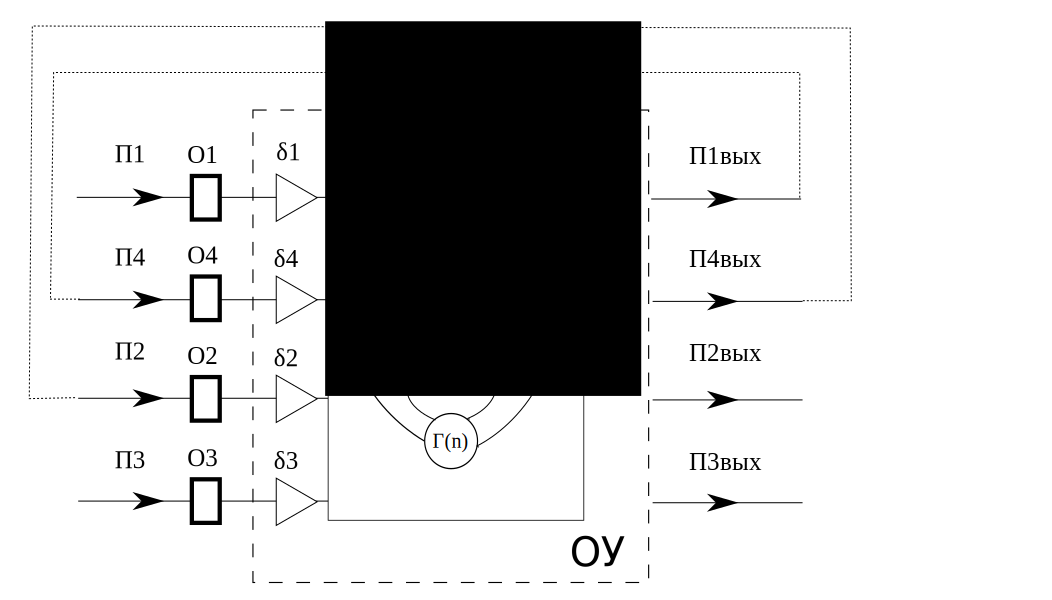
\includegraphics[width=\textwidth]{SystemScheme.pdf} % or {1.eps} in case of EPS format of the picture
    \caption {Scheme of the queuing system as a cybernetic control system}
    \label{SystemScheme}
\end{figure}

In order to describe the server behavior we fix positive integers $d$, $n_0$, $n_1$, $\ldots$,
$n_d$ and we introduce a finite set $\Gamma=\{\Gamma^{(k,r)} \colon k=0,1,\ldots,d; r=1,2,\ldots
n_k\}$ of states server can reside in. At the state $\Gamma^{(k,r)}$ sever stays during constant
time $T^{(k,r)}$. Define disjoint subsets $\Gamma^{\mathrm{I}}$, $\Gamma^{\mathrm{II}}$,
$\Gamma^{\mathrm{III}}$, and $\Gamma^{\mathrm{IV}}$ of $\Gamma$ as follows.  In the state $\gamma
\in \Gamma^{\mathrm{I}}$ only customers from the queues $O_1$, $O_2$ and $O_4$ are serviced.  In the
state $\gamma \in \Gamma^{\mathrm{II}}$ only customers from the queues $O_2$ and $O_4$ are serviced.
In the state $\gamma \in \Gamma^{\mathrm{III}}$ only customers from queues $O_1$, $O_3$, and $O_4$
are serviced.  In the state $\gamma \in \Gamma^{\mathrm{IV}}$ only customers from queues $O_3$ and
$O_4$ are serviced.  We assume that $\Gamma = \Gamma^{\mathrm{I}} \cup \Gamma^{\mathrm{II}} \cup
\Gamma^{\mathrm{III}} \cup \Gamma^{\mathrm{IV}}$. Set also ${}^1\Gamma=\Gamma^{\mathrm{I}} \cup
\Gamma^{\mathrm{III}}$, ${}^2\Gamma=\Gamma^{\mathrm{I}} \cup \Gamma^{\mathrm{II}}$,
${}^3\Gamma=\Gamma^{\mathrm{III}} \cup \Gamma^{\mathrm{IV}}$.

The server changes its state according to the following rules. We call a set $C_k = \{\Gamma^{(k,r)}
\colon r=1,2,\ldots n_k\}$ the $k$-th cycle, $k=1$, $2$, $\ldots$, $d$. For $k=0$ the state
$\Gamma^{(0,r)}$ with $r=1$, $2$, $\ldots$, $n_0$ is called a prolongation state. Put $r \oplus_k 1
= r+1$ for $r<n_k$, and $r \oplus_k 1 = 1$ for $r=n_k$ ($k = 0$, $1$, $\ldots$, $d$). In the cycle
$C_k$ we select a subset $C_k^{\mathrm{O}}$ of input states, a subset $C_k^{\mathrm{I}}$ of output
states, and a subset $C_k^{\mathrm{N}} = C_k \setminus (C_k^{\mathrm{O}} \cup C_k^{\mathrm{I}})$ of
neutral states.  After the state $\Gamma^{(k,r)} \in C_k\setminus C_k^{\mathrm{O}}$ the server
switches to the state $\Gamma^{(k,r \oplus_k 1)}$ within the same cycle $C_k$.  After the state
$\Gamma^{(k,r)}$ in $C_k^{\mathrm{O}}$ the server switches to the state $\Gamma^{(k,r \oplus_k 1)}$
if number of customers in the queue $O_3$ at switching instant is greater than a predetermined
threshold $L$.  Otherwise, is the number of customers in the queue $O_3$ is less than or equals $L$
then the new state is the prolongation one $\Gamma^{(0,r_1)}$ where $r_1=h_1(\Gamma^{(k,r)})$ and
$h_1(\cdot)$ is a given mapping of $\bigcup_{k=1}^d C_k^{\mathrm{O}}$ into $\{1,2,\ldots,
n_0\}$.  After the state $\Gamma^{(0,r)}$ if the number of customers in $O_3$ is not above $L$ the
state of the same type $\Gamma^{(0,r_2)}$ is chosen where $r_2=h_2(r)$ and $h_2(\cdot)$ is a given
mapping of the set $\{1,2, \ldots, n_0\}$ into itself; in the other case the new state is
$\Gamma^{(k,r_3)} \in C_k^{\mathrm{I}}$ where $\Gamma^{(k,r_3)}=h_3(r)$ and $h_3(\cdot)$ is a 
given mapping of  $\{1,2, \ldots, n_0\}$ to $\bigcup_{k=1}^d C_k^{\mathrm{I}}$. We assume
that each prolongation state $\Gamma^{(0,r)}$ belongs to the set ${}^2 \Gamma$ and that relations
$C_k^\mathrm{O}\subset {}^2 \Gamma$ and $C_k^\mathrm{I}\subset {}^3 \Gamma$ hold. We also assume
that all the cycles have exactly one input and output state. Finally, we assume that all the
prolongation states make a cycle, that is  $h_2(r)=r\oplus_0 1$. Putting all together, we introduce
a function which formalizes the server state changes:
\begin{equation}
h(\Gamma^{(k,r)},y) = 
\begin{cases}
\Gamma^{(k,r \oplus_k 1)}&  \text{ if  $\Gamma^{(k,r)}\in C_k\setminus C_k^{\mathrm{O}}$ or $(\Gamma^{(k,r)}\in C_k^{\mathrm{O}}) \wedge (y>L)$;}\\
\Gamma^{(0,h_1(\Gamma^{(k,r)}))}&  \text{ if  $\Gamma^{(k,r)}\in C_k^{\mathrm{O}}$ and $y\leqslant L$;}\\
\Gamma^{(0,r \oplus_0 1)}&  \text{ if $k=0$ and $y\leqslant L$;}\\
h_3(r)&  \text{ if  $k=0$ and $y > L$.}
\end{cases}
\label{hLaw}
\end{equation}

In general, service durations of different customers can be dependent and may have different laws of
probability distributions. So, saturation flows will be used to define the service process. A
saturation flow $\Pi^{\mathrm{\text{sat}}}_j$, $j \in \{1,2,3,4\}$, is defined as a virtual output
flow under the maximum usage of the server and unlimited number of customer in the queue $O_j$. The
saturation flow $\Pi^{\mathrm{\text{sat}}}_j$, $j\in \{1,2,3\}$ contains a non-random number
$\ell({k,r,j)}\geqslant0$ of customers in the server state $\Gamma^{(k,r)}$. In particular,
$\ell({k,r,j)}\geqslant1$ for $\Gamma^{(k,r)}\in{}^j\Gamma$ and $\ell({k,r,j)}=0$ for
$\Gamma^{(k,r)}\not\in{}^j\Gamma$. Let $\mathbb{Z}_+$ be
the set of non-negative integer numbers. If the queue $O_4$ contains $x \in \mathbb{Z}_+$ customers
the saturation flow $\Pi^{\mathrm{\text{sat}}}_4$ also contains the $x$ customers.  Finally, in the
state $\Gamma^{(k,r)}$ every customer from queue $O_4$ with probability $p_{k,r}$ and independently
of others ends servicing and joins $\Pi_2$ to go to $O_2$. With the complementary probability
$1-p_{k,r}$ the customer stays in $O_4$ until the next time slot. In the next time slot it repeats
its attempt to join $\Pi_2$ with a proper probability.

A real-life example of just described queuing system is a tandem of two consecutive crossroads
(Fig. \ref{crossroads}).
\begin{figure}[h!]
   \centering
    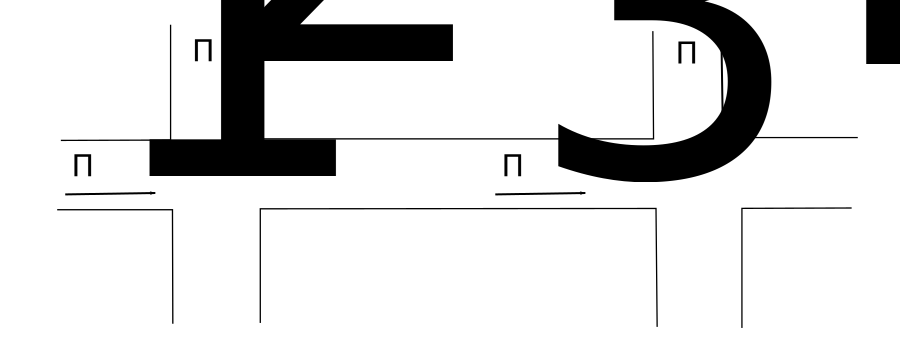
\includegraphics[width=\textwidth]{Crossroads.pdf} 
    \caption {A tandem of crossroads, the physical interpretation of the queuing system under study}
    \label{crossroads}
\end{figure}
The input flows are flows of vehicles. The flows $\Pi_1$ and $\Pi_5$ at the first crossroad are
conflicting; $\Pi_2$ and $\Pi_3$ at the second crossroad are also conflicting. Every vehicle from
the flow $\Pi_1$ after passing first road intersection joint the flow $\Pi_4$ and enters the queue
$O_4$. After some random time interval the vehicle arrives to the next road intersection. Such a pair
of crossroads is an instance of a more general queuing model described above.

\section{Mathematical model}
The queuing system under investigation can be regarded as a cybernetic control system what helps to
rigorously construct a formal stochastic model~\cite{z:2012}. The scheme of the control system is
shown in Fig.~\ref{SystemScheme}. There are following blocks present in the scheme: 1)~the external
environment with one state; 2) input poles of the first type~--- the input flows $\Pi_1$, $\Pi_2$,
$\Pi_3$, and $\Pi_4$; 3) input poles of the second type~--- the saturation flows
$\Pi^{\mathrm{\text{sat}}}_1$, $\Pi^{\mathrm{\text{sat}}}_2$, $\Pi^{\mathrm{\text{sat}}}_3$, and
$\Pi^{\mathrm{\text{sat}}}_4$; 4)~an external memory~--- the queues $O_1$, $O_2$, $O_3$, and $O_4$;
5)~an information processing device for the external memory~--- the queue discipline units
$\delta_1$, $\delta_2$, $\delta_3$, and $\delta_4$; 6) an internal memory --- the server (OY); 7)~an
information processing device for internal memory~--- the graph of server state transitions;
8)~output poles~--- the output flows $\Pi^{\mathrm{\text{out}}}_1$, $\Pi^{\mathrm{\text{out}}}_2$,
$\Pi^{\mathrm{\text{out}}}_3$, and $\Pi^{\mathrm{\text{out}}}_4$.  The coordinate of a block is
its number on the scheme.

Let us  introduce the following variables and elements along with their
value ranges. To fix a discrete time scale consider the epochs $\tau_0=0$, $\tau_1$, $\tau_2$,
$\ldots$ when the server changes its state. Let $\Gamma_i\in\Gamma$ be the server state
during the interval $(\tau_{i-1};\tau_i]$, $\varkappa_{j,i} \in \mathbb{Z}_+ $ be the number of customers in
the queue $O_j$ at the instant $\tau_i$, $\eta_{j,i} \in \mathbb{Z}_+$ be the number of customers
arrived into the queue $O_j$ from the flow $\Pi_j$ during the interval $(\tau_{i};\tau_{i+1}]$, $\xi_{j,i} \in
\mathbb{Z}_+$ be the number of customers in the saturation flow $\Pi^{\mathrm{\text{sat}}}_j$ during
the interval $(\tau_{i};\tau_{i+1}]$, $\overline{\xi}_{j,i}\in \mathbb{Z}_+$ be the actual number of 
serviced customers from the queue  $O_j$ during the interval $(\tau_{i};\tau_{i+1}]$, $j\in
\{1,2,3,4\}$.

The server changes its state according to the following rule:
\begin{equation}
\Gamma_{i+1}=h(\Gamma_i,\varkappa_{3,i})
\label{gammaFunc}
\end{equation}
where the mapping $h(\cdot,\cdot)$ is defined by Formula~\eqref{hLaw}.
To determine the duration $T_{i+1}$ of the next time slot it useful to introduce a mapping
$h_T(\cdot,\cdot)$ by
\begin{equation*}
T_{i+1}=h_T(\Gamma_i,\varkappa_{3,i})= T^{(k,r)}\quad  \text{ where $ \Gamma^{(k,r)}=\Gamma_{i+1}=h(\Gamma_i,\varkappa_{3,i})$.}
\end{equation*}
A functional relation
\begin{equation}
\overline{\xi}_{j,i}=\min\{\varkappa_{j,i}+\eta_{j,i},\xi_{j,i}\}, \quad j\in \{1,2,3\},
\label{saturationEq}
\end{equation}
between $\overline{\xi}_{j,i}$ and $\varkappa_{j,i}$, $\eta_{j,i}$, $\xi_{j,i}$ describes the
service strategy. Further, since
\begin{equation*}
\varkappa_{j,i+1}=\varkappa_{j,i}+\eta_{j,i}-\overline{\xi}_{j,i}, \quad  j\in \{1,2,3\},
\end{equation*}
and due to \eqref{saturationEq} it follows that 
\begin{equation}
\varkappa_{j,i+1}=\max\{{0,\varkappa_{j,i}+\eta_{j,i}-\xi_{j,i}}\}, \quad j\in \{1,2,3\}.
\label{queuesFunc}
\end{equation}

We also have from  the  problem settings the following relations for the flow $\Pi_4$:
\begin{equation}
\eta_{4,i} = \min\{\xi_{1,i}, \varkappa_{1,i}+\eta_{1,i}\}, \quad \varkappa_{4,i+1}=\varkappa_{4,i}+\eta_{4,i}-\eta_{2,i}, \quad \xi_{4,i} = \varkappa_{4,i}.
\label{FourthFunc}
\end{equation}

Put $\varkappa_i=(\varkappa_{1,i},\varkappa_{2,i},\varkappa_{3,i},\varkappa_{4,i})$. The non-local
description of the input and saturation flows consists in specifying particular features of the
 conditional probability distribution of selected discrete components
$\eta_i=(\eta_{1,i},\eta_{2,i}, \eta_{3,i}, \eta_{4,i})$ and $\xi_i=(\xi_{1,i}, \xi_{2,i},
\xi_{3,i}, \xi_{4,i})$ of marked point processes $\{(\tau_i, \nu_i, \eta_i); i\geqslant 0\}$ and
$\{(\tau_i, \nu_i, \xi_i); i\geqslant 0\}$ with marks $\nu_i = (\Gamma_i;\varkappa_i)$. Let
$\varphi_1(\cdot,\cdot)$ and $\varphi_3(\cdot,\cdot)$ be defined by series expansions
\begin{equation*}
\sum_{\nu=0}^{\infty} z^\nu\varphi_j(\nu,t) = \exp\{\lambda_j t (f_j(z)-1)\}
\end{equation*}
with functions where $f_j(z)$ defined by \eqref{GeneratingFunc}, $j \in \{1,3\}$. The function
$\varphi_j(\nu,t)$ equals the probability of  $\nu=0$, $1$, $\ldots${} arrivals in the flow
$\Pi_j$ during time $t \geqslant 0$. If $\nu < 0$ the value of $\varphi_j(\nu,t)$ is set to
zero. Define function $\psi(\cdot,\cdot,\cdot)$ by
\begin{equation*}
\psi(k;y,u)=C_y^k u^k (1-u)^{y-k}.	
\end{equation*}
Then $\psi(k;y,p_{k,r})$ is the probability of $k$ arrival from flow $\Pi_2$ given the queue $O_4$
contains $y$ customers and the server state is $\Gamma^{(k,r)}$. For values $k\not\in\{0, 1, \ldots,
y\}$ the value of $\psi(k;y,u)$ is set to zero.

Let $a=(a_1, a_2, a_3, a_4) \in \mathbb{Z}_+^4$ and $x=(x_1, x_2, x_3, x_4) \in
\mathbb{Z}_+^4$. If the mark value is 
$\nu_i=(\Gamma^{(k,r)}; x)$ then the probability $\varphi(a,k,r,x)$ of simultaneous
equalities  $\eta_{1,i}=a_1$, $\eta_{2,i}=a_2$, $\eta_{3,i}=a_3$, $\eta_{4,i}=a_4$ according the the
problem statement is
\begin{equation*}
\varphi_1(a_1,h_T(\Gamma^{(k,r)},x_3)) \cdot \psi(a_2,x_4, p_{\tilde{k},\tilde{r}}) \cdot \varphi_3(a_3,h_T(\Gamma^{(k,r)},x_3))
\cdot \delta_{a_4,\min{\{\ell{(\tilde{k},\tilde{r},1)}, x_1+a_1}\}}
\label{conditionProbOne}
\end{equation*}
where $\Gamma^{(\tilde{k},\tilde{r})}=h(\Gamma^{(k,r)},x_3)$ and $\delta_{i,j}$ is the Kroneker's delta:
\begin{equation*}
\delta_{i,j}=\begin{cases} 1 &\text{ if $i=j$,}\\0 &\text{ if $i\neq j$.}
\end{cases}
\end{equation*}
Let $b=(b_1, b_2, b_3, b_4) \in \mathbb{Z}_+^4$. The probability $\zeta(b, k, r, x)$  of
simultaneous equalities $\xi_{1,i}=b_1$, $\xi_{2,i}=b_2$, $\xi_{3,i}=b_3$, $\xi_{4,i}=b_4$ given the
fixed label value $\nu_i=(\Gamma^{(k,r)}; x)$ is
\begin{equation*}
\delta_{b_1,\ell(\tilde{k},\tilde{r},1)} \cdot \delta_{b_2,\ell(\tilde{k},\tilde{r},2)} \cdot
\delta_{b_3,\ell(\tilde{k},\tilde{r},3)} \cdot \delta_{b_4,x_4}.
\label{conditionProbTwo}
\end{equation*}

The assumptions on statistical properties of some blocks and function relations between blocks are
not contradicting and sufficient to construct a formal probability model, as the following theorem
first proven in \cite{k:z:02:2015} demonstrates.
\begin{thm}\label{thm1}
  Choose $\gamma_0=\Gamma^{(k_0,r_0)}\in \Gamma$ and $x^0=(x_{1,0},x_{2,0}, x_{3,0},x_{4,0})\in
  \mathbb{Z}_+^4$.  There exists a probability space $(\Omega, {\cal F}, \Pr(\cdot))$, random
  variables $\eta_{j,i}=\eta_{j,i}(\omega)$, $\xi_{j,i}=\xi_{j,i}(\omega)$,
  $\varkappa_{j,i}=\varkappa_{j,i}(\omega)$, and random elements $\Gamma_i=\Gamma_i(\omega)$,
  $i\geqslant 0$, $j\in \{1, 2, 3, 4\}$  defined on this space, such that: 1)~equalities
  $\Gamma_0(\omega) = \gamma_0$ and $\varkappa_0(\omega)=x^0$ hold; 2)~relations
  \eqref{gammaFunc}, \eqref{queuesFunc}, \eqref{FourthFunc} hold; 3)~for any $a$, $b$,
  $x^t=(x_{1,t},x_{2,t},x_{3,t},x_{4,t}) \in \mathbb{Z}_+^4$, $\Gamma^{(k_t,r_t)} \in \Gamma$, $t =
  1, 2, \ldots$ the joint conditional probability distribution of vectors $\eta_i$ and $\xi_i$ has the form
  \begin{multline*}
    \Pr \biggl(\Bigl\{ \omega \colon \eta_i(\omega) = a, \xi_i(\omega)=b\Bigr\}\,
    \bigg|\bigcap_{t=0}^{i}\Bigl\{\omega\colon \Gamma_t(\omega)=\Gamma^{(k_t,r_t)},
    \varkappa_t(\omega)=x^t\Bigr\}\biggr)
    \\ =    \varphi(a,k_i,r_i,x^i) \cdot \zeta(b,k_i,r_i,x^i).
    \label{ProbablititiesToProve}
  \end{multline*}
\label{myTheorem}
\end{thm}

From now on we focuse on low-priority customers in the queue $O_3$. 

\section{The low-priority queue}

Here we will consider the stochastic sequence
\begin{equation}
\label{eq:theMC}
\{(\Gamma_i(\omega), \varkappa_{3, i}(\omega)); i =0, 1, \ldots\}
\end{equation}
which includes the number of low-priority customers $\varkappa_{3, i}(\omega)$ in the queue $O_3$.  In this
section we will report several results concerning this stochastic sequence.

\begin{thm}
  Let $\Gamma_0(\omega)=\Gamma^{(k,r)}\in \Gamma$ and $\varkappa_{3,0}(\omega)=x_{3,0}\in
  \mathbb{Z}_+$ be fixed. Then the stochastic sequence~\eqref{eq:theMC} is a
  homogeneous denumerable Markov chain.
\end{thm}

\begin{thm}
Let $x_3$, $\tilde{x}_3\in \mathbb{Z}_+$ and $\Gamma^{(k,r)}$,
$\Gamma^{(\tilde{k},\tilde{r})}=h(\Gamma^{(k,r)},x_3) \in \Gamma$. Then the transition probabilities
of the  Markov chain~\eqref{eq:theMC}  are
\begin{multline*}
\Pr (\{\omega\colon
\Gamma_{i+1}(\omega)=\Gamma^{(\tilde{k},\tilde{r})},\varkappa_{3,i+1}(\omega)=\tilde{x}\}\mid\{\omega\colon
\Gamma_{i}(\omega)=\Gamma^{(k,r)},\varkappa_{3,i}(\omega)=x\}) 
\displaybreak[0]
\\ = (1-\delta_{\tilde x_3, 0})\cdot \varphi\Bigl(\tilde x_3+ \ell(\tilde k, \tilde r, 3)-x_3, h_T\bigl(
\Gamma^{(\tilde k, \tilde r)}, x_3\bigr)\Bigr) 
\displaybreak[0]
\\ +  \delta_{\tilde x_3, 0} \sum_{a=0}^{ \ell(\tilde k, \tilde r, 3)-x_3} \varphi_3\Bigl(a, h_T\bigl(
\Gamma^{(\tilde k, \tilde r)}, x_3\bigr)\Bigr).
\label{transitionToProve:three}
\end{multline*}
\end{thm}

The last theorem clarifies which states of the Markov chain $\{(\Gamma_i, \varkappa_{3, i}); i \geqslant
0\}$ are essential. To make a complete classification we introduce sets
\begin{align*}
  S^3_{0,r} = & 
  \biggl\{
  (\Gamma^{(0,r)},x_3) \colon \; x_3\in Z_+,\; L \geqslant x_3 > L - \max\limits_{k=1, 2,
    \ldots, d}
  \biggl\{ \sum_{t=0}^{n_k} \ell({k,t,3}) \biggl\}\biggl\}, 
  \quad 1 \leqslant r \leqslant n_0, \\
  S^3_{k,r} = & 
  \biggl\{
  (\Gamma^{(k,r)},x_3) \colon \; x_3\in Z_+,\; x_3 > L - \sum_{t=0}^{r-1} \ell({k,t,3})
  \biggr\}, 
  \quad 1 \leqslant k \leqslant d, \quad 1 \leqslant r \leqslant n_k.
\end{align*}

\begin{thm}
The set of essential states of the Markov chain $\{(\Gamma_i, \varkappa_{3, i}); i \geqslant 0\}$  consists of sets $\bigcup\limits_{1 \leqslant r \leqslant n_0}S^3_{0,r}$ and $\bigcup\limits_{\substack{1 \leqslant k \leqslant d\\ 1 \leqslant r \leqslant n_k}} S^3_{k,r}\:$.
\end{thm}

As before, let $\Gamma^{(k,r)}\in \Gamma$ and $x_3 \in Z_+$. Denote by 
$H_{-1}(\Gamma^{(k,r)}, x_3)$ the set of all server states $\gamma$ such that $h(\gamma, x_3) =
\Gamma^{(k,r)}$ and put $r \ominus_k 1
= r-1$ for $n_k \geqslant r>0$, and $r \ominus_k 1 = n_k$ for $r=0$ ($k = 0$, $1$, $\ldots$, $d$).
Then formula \eqref{hLaw} makes it possible to define  the mapping $H_{-1}(\Gamma^{(k,r)}, x_3)$ explicitly:
\begin{equation}
H_{-1}(\Gamma^{(k,r)}, x_3) = 
\begin{cases}
\bigl\{\Gamma^{(k_1,r_1)}, \Gamma^{(0,r\ominus_0 1)}\bigr\}&  \text{ if  $(k=0) \wedge (x_3 \leqslant L)$,}\\
\bigl\{\Gamma^{(k,r\ominus_k 1)}, \Gamma^{(0,r_2)}\bigr\}&  \text{ if  $(\Gamma^{(k,r)}\in C_k^{\mathrm{I}})
  \wedge (x_3>L)$,}\\ 
\bigl\{\Gamma^{(k,r\ominus_k 1)}\bigr\}&  \text{ if  $(\Gamma^{(k,r)}\in C_k^{\mathrm{O}}) \vee (\Gamma^{(k,r)}\in C_k^{\mathrm{N}})$;}\\
\varnothing&  \text{ if  $(k = 0)\wedge  (x_3>L)$}\\
 & \qquad \text{ or $(\Gamma^{(k,r)}\in C_k^{\mathrm{I}}) \wedge (x_3\leqslant L)$}
\end{cases}
\end{equation}
where $h_1(\Gamma^{(k_1,r_1)})=r$ and $h_3(r_2)=\Gamma^{(k,r)}$.

Let's define for $\gamma \in \Gamma$ and $x_3 \in Z_+$ values
\begin{equation*}
Q_{3,i}(\gamma,x) = \Pr(\{\omega\colon \Gamma_{i}(\omega)=\gamma, \varkappa_{3,i}(\omega)=x_3\}).
\end{equation*}
Suppose $k$ and $r$ are such that $\Gamma^{(k,r)}\in \Gamma$. Let's define the partial probability generating functions 
\begin{gather*}
\mathfrak{M}^{(i)}(k,r,v) = \sum_{w=0}^{\infty} Q_{3,i}(\Gamma^{(k,r)},w) v^w,\qquad
\Phi^{(i)}(k,r,v) =  \sum_{x_3=0}^{\infty} \sum_{\gamma \in H_{-1}(\Gamma^{(k,r)},x_3)} Q_{3,i}(\gamma,x_3) v^{x_3},\\
q_{k,r}(v) = v^{-\ell(k,r,3)}\sum_{w=0}^{\infty} \varphi_3(w,T^{(k,r)})v^w.
\end{gather*}

\begin{thm}
Let $\tilde{\gamma}=\Gamma^{(\tilde{k},\tilde{r})} \in \Gamma$. The following recurrent w.r.t. $i
\geqslant 0$ relations take place for the  partial probability generating functions:
\begin{multline*}
\mathfrak{M}^{(i+1)}(\tilde{k},\tilde{r},v) =  
q_{\tilde k, \tilde r}(v)
\Phi^{(i)}(\tilde{k},\tilde{r},v)+\sum_{x_3=0}^{\ell(\tilde{k},\tilde{r},3)}\sum_{\gamma \in H_{-1}(\tilde{\gamma},x_3)} Q_{3,i}(\gamma,x_3) \sum_{a=0}^{\ell(\tilde{k},\tilde{r},3) - x_3} \varphi_3(a,T^{(\tilde{k},\tilde{r})}) - \\
- \sum_{x_3=0}^{\ell(\tilde{k},\tilde{r},3)}  \sum_{\gamma \in H_{-1}(\tilde{\gamma},x_3)} Q_{3,i}(\gamma,x_3) v^{x_3-\ell(\tilde{k},\tilde{r},3)}  \sum_{w=0}^{\ell(\tilde{k},\tilde{r},3) + 1 -x_3}\varphi_3(w,T^{(\tilde{k},\tilde{r})}) v^w.
\label{markk_proiz}
\end{multline*}
\end{thm}

\section{Acknowledgments}

This work was fulfilled as a part of State Budget Research and Development program No.~01201456585
``Mathematical modeling and analysis of stochastic evolutionary systems and decision processes'' of
N.I. Lobachevsky State University of Nizhni Novgorod and was supported by State Program ``Promoting
the competitiveness among world's leading research and educational centers''


\begin{thebibliography}{99}
\bibitem{n:f:p:1968} Neimark Yu.~I., Fedotkin M.~A., Preobrazhenskaja A.~M. Operation of an automate
  with feedback controlling traffic at an intersection~// Izvestija of USSR Academy of Sciences,
  Technical Cybernetic. 1968. No.~5. P.~129--141.
\bibitem{f:1977} %
  Fedotkin M.~A. On a class of stable algorithms for control of conflicting flows or arriving
  airplanes~// Problems of control and information theory. 1977. V.~6, No.~1. P.~13--22.
\bibitem{f:1977-1} %
  Fedotkin M.~A. Construction of a model and investigation of nonlinear algorithms for control of
  intense conflict flows in a system with variable structure of servicing demands. I~// Lithuanian
  mathematical journal. 1977. V.~17, No.~1. P.~129--137.
\bibitem{l:f:2000}%
  Litvak N.~V., Fedotkin M.~A. A probabilistic model for the
  adaptive control of conflict flows~// Automation and Remote Control. 2000. V. 61, No. 5. P.~777--784.
\bibitem{p:f:2008}%
  Proidakova E.V., Fedotkin M.A. Control of output flows in the system with cyclic servicing and
  readjustments~// Automation and remote control. 2008. V. 69, No. 6. P.~993--1002.
\bibitem{a:b:2010}%
  Afanasyeva L.~G., Bulinskaya E.~V. Mathematical models of transport systems based on queueing
  theory~// Trudy of Moscow Institute of Physocs and Technology. 2010. No.~4. P.6--21. 
\bibitem{y:l:1985} %
  Yamada K., Lam T.~N. Simulation analysis of two adjacent traffic signals~// Proceedings of the
  17th winter simulation conference. ACM, New York. 1985. P.~454--464.
\bibitem{z:2012}%
  Zorin A.V. Stability of a tandem of queueing systems with Bernoulli noninstantaneous transfer of
  customers~// Theory of Probability and Mathematical Statistics. 2012. V.~84. P.~173-188.
\bibitem{k:z:02:2015} %
  Kocheganov V.~M., Zorine A.V. Probabilistic model of tandem of queuing systems under cyclic
  control with prolongations~// Proceedings of Internation conference ``Probability theory, stochastic processes, mathematical statistics
  and applications'' (Minsk, Feb. 23--26 2015). 2015. P.~94-99.
\end{thebibliography}
\end{document}
